Accounting for power and temperature is key to achieving effectiveness,
efficiency, and robustness. However, the power and temperature characteristics
of the system under development are difficult to describe mathematically or
algorithmically. Modern systems are complex, and many aspects are inherently
uncertain to the designer due to such phenomena as process variation
\cite{chandrakasan2000}, aging \cite{coskun2006}, and varying workload.

The above concern is particularly hard to address from a theoretical standpoint;
it can be better dealt with taking a more pragmatic approach, namely, making use
of runtime data. Assuming that the system provides mechanisms for profiling and
monitoring, direct or indirect power and temperature readings are an invaluable
source of information for making proactive power- and temperature-aware
decisions \cite{chaudhry2015, coskun2008}.

\begin{figure}[b]
  \centering
  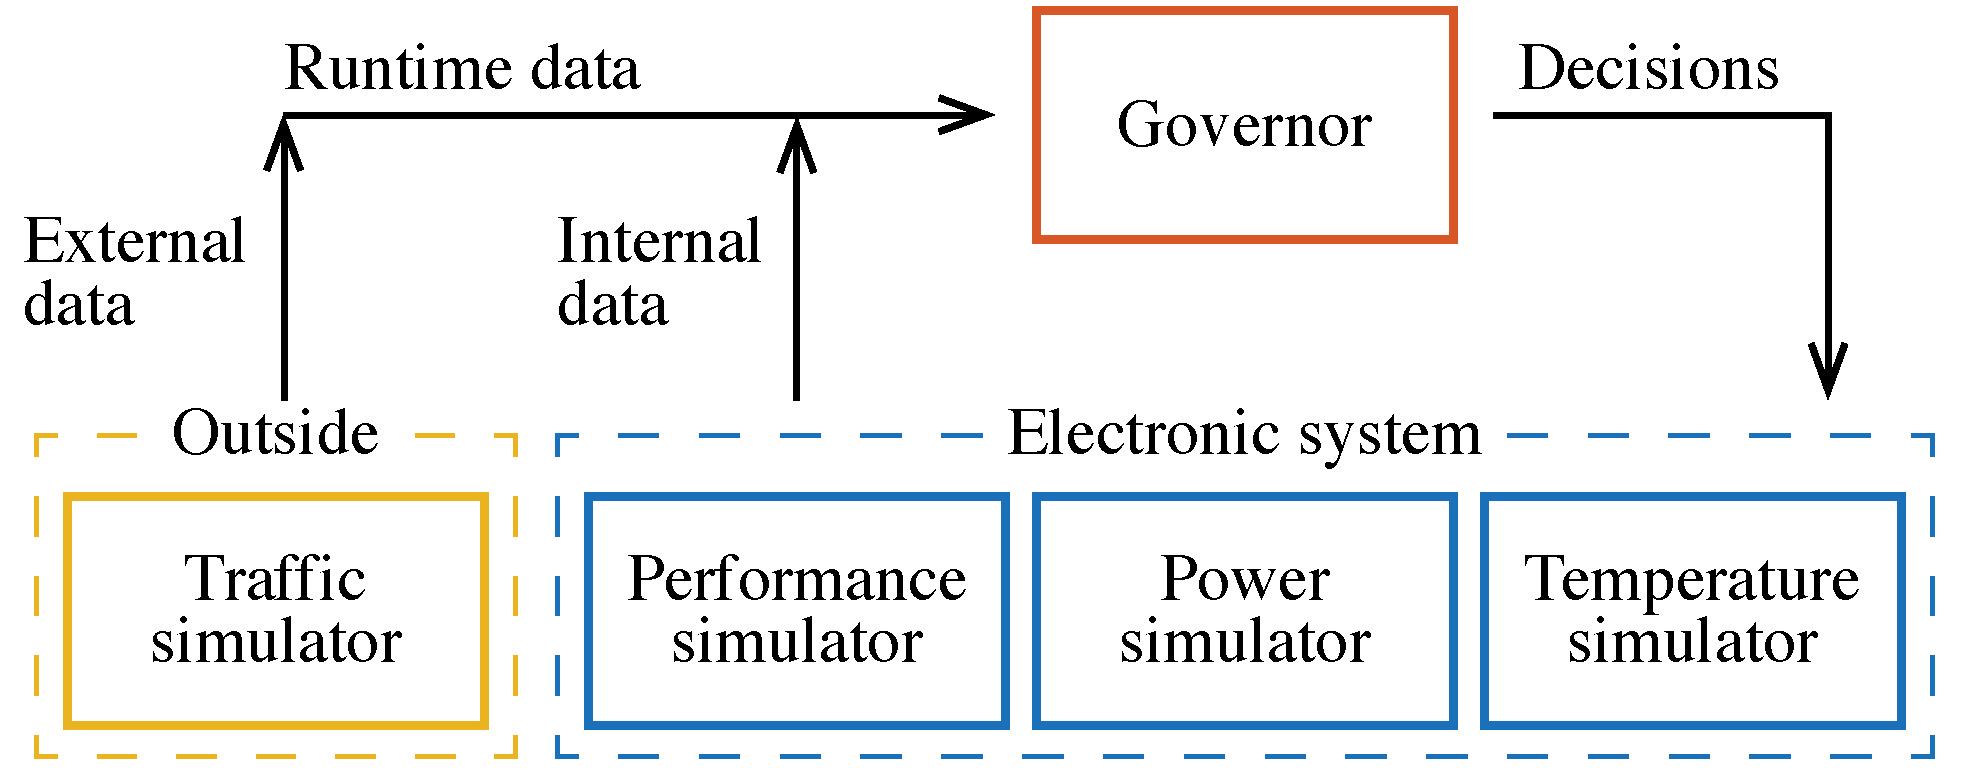
\includegraphics[width=1.0\columnwidth]{include/assets/figures/development.pdf}
  \caption{
    A research environment for developing a resource manager of an electronic
    system. The right dashed box should be understood at a single module, and
    the corresponding arrows should be treated accordingly.
  }
  \flab{development}
\end{figure}

Acting proactively requires forecasting the future by learning from the past,
which is typically accomplished by virtue of statistics and adjacent fields such
as machine learning \cite{bishop2006}. Regardless of the learning technique
utilized, the technique needs data to learn from. In the case of a platform that
does not exist yet, such data can be obtained from computer simulators.
Simulators are extensively utilized even when an existing platform is concerned
since it might not be available or might not be an appropriate place for
experimentation, which is common in research. Therefore, a typical research
environment is composed of a number of simulators. To give an example, the
illustration given in \fref{development} depicts a potential environment for
developing a governor of an electronic system.

Computer simulators, however, fall short when it comes to complex systems: and
it might take days for a state-of-the-art simulator to simulate a short, in
wall-clock time, program. This scheme is not affordable for designing
data-driven techniques as they require many simulations with potentially large
payloads.

In conclusion, real data are rarely or unwillingly available, and simulation
data are prohibitively time consuming to obtain, which limits the exploration of
data-driven techniques. The need for alternative sources of high-quality data is
prominent.
